\documentclass[t]{beamer}
\usepackage[utf8]{inputenc} % to be able to type unicode text directly
\usepackage{inconsolata} % for a nicer (e.g. non-courier) tt family font

\usepackage{graphicx} % to include figures
\usepackage{hyperref,url} % to make clickable hyperlinks
\usepackage{minted} % for code insets
\usepackage{array} %
\usepackage{bbm} % for blackboard 1

\usepackage{tikz}

\usepackage{soul}
\usepackage{cancel}
\renewcommand{\CancelColor}{\color{red}}

\colorlet{darkgreen}{black!50!green}
\colorlet{ddarkgreen}{black!75!green}
\colorlet{darkred}{black!50!red}
\definecolor{ipol}{rgb}{.36,.29,.65}
\usecolortheme[named=ipol]{structure}
\definecolor{term}{rgb}{.9,.9,.9}

\newcommand{\reference}[1] {{\scriptsize \color{gray}  #1 }}
\newcommand{\referencep}[1] {{\tiny \color{gray}  #1 }}
\newcommand{\unit}[1] {{\tiny \color{gray}  #1 }}

\def\R{\mathbf{R}}
\def\F{\mathcal{F}}
\def\x{\mathbf{x}}
\def\u{\mathbf{u}}
\def\FFT{\mathtt{FFT}}
\def\IFFT{\mathtt{IFFT}}
\DeclareMathOperator*{\argmin}{arg\,min}

% disable spacing around verbatim
\usepackage{etoolbox}
\makeatletter
\preto{\@verbatim}{\topsep=0pt \partopsep=0pt }
\makeatother

\mode<presentation>
\setbeamercolor*{author in head/foot}{parent=none}
\setbeamercolor*{title in head/foot}{parent=none}
\setbeamercolor*{date in head/foot}{parent=none}
\defbeamertemplate*{footline}{infoline theme}
{
  \leavevmode%
  \hfill\color{darkgreen}
   \insertframenumber{} / \inserttotalframenumber\hspace*{2ex}
  \vskip0pt%
}

\makeatletter
\newcommand\SoulColor{%
  \let\set@color\beamerorig@set@color
  \let\reset@color\beamerorig@reset@color}
\makeatother
\newcommand<>{\St}[1]{\only#2{\SoulColor\st{#1}}}
\setstcolor{red}

\mode<all>
\setbeamertemplate{navigation symbols}{}

%\setbeamersize{text margin left=1em,text margin right=1em} (does not work)
%\setbeamersize{text margin left=1em}


\begin{document}

\begin{frame}[plain,fragile]
\begin{verbatim}








                VECTOR CALCULUS ON GRAPHS









Enric Meinhardt-Llopis
GTTI 30/11/2016
\end{verbatim}
%	\titlepage
%	\begin{columns}
%		\begin{column}{0.4\linewidth}
%			Enric Meinhardt-Llopis\\
%			CMLA, ENS--Cachan\\
%			%IPOL (Image Processing On Line)\\
%			{\small\color{ipol}\url{http://ipol.im}}
%		\end{column}
%		\begin{column}{0.6\linewidth}
%			\includegraphics[width=4em]{f2/logocmla.jpg}$\quad$%
%			\includegraphics[width=6em]{f2/logoens.jpg}$\quad$%
%			\includegraphics[width=4em]{f2/logoipol.jpg}$\quad$%
%		\end{column}
%	\end{columns}
\end{frame}

\begin{frame}[fragile]\begin{verbatim}CONCLUSION
==========


1. The design of ad-hoc finite difference schemes
is not a worthwhile human activity.

2. Instead, model your problem in the continuous domain
and use the correspondence between graphs and vector calculus.

3. Octave/Matlab is *very* smart when dealing with
sparse matrices.  Write your code as short as possible.
\end{verbatim}

\vspace{2.5em}\pause

\tiny\tt
\begin{tabular}{cccc}
	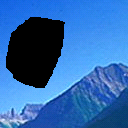
\includegraphics[width=0.18\linewidth]{lenasky/crop_lenasky_boundary.png} &
	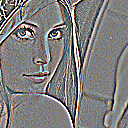
\includegraphics[width=0.18\linewidth]{lenasky/crop_minuslap.png} &
	%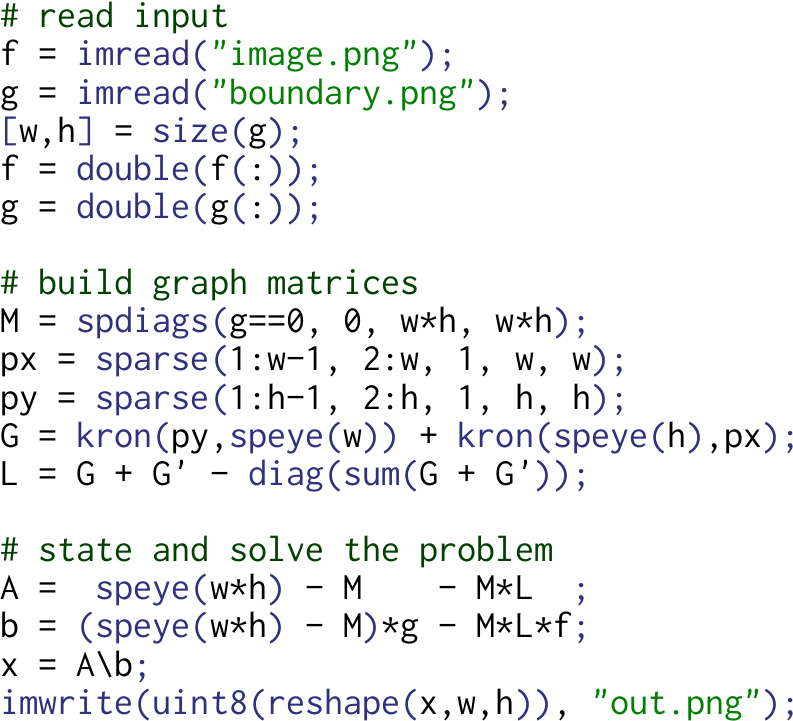
\includegraphics[width=0.21\linewidth]{lenasky/mini2.png} &
	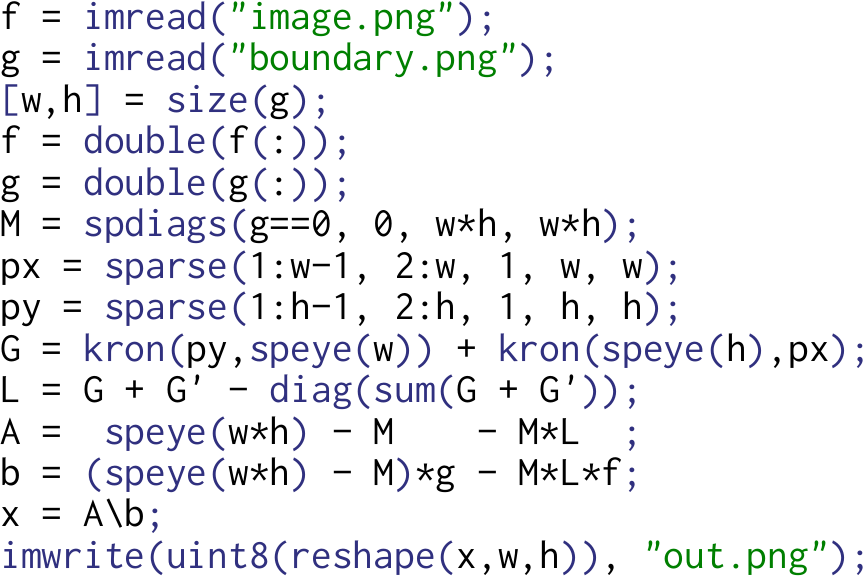
\includegraphics[width=0.28\linewidth]{lenasky/miniercode.png} &
	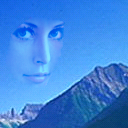
\includegraphics[width=0.18\linewidth]{lenasky/crop_result.png} \\
	boundary condition &
	laplacian &
	poisson solver &
	result \\
\end{tabular}
\end{frame}


\begin{frame}[fragile]\begin{verbatim}Contents
========


1. Some horrific finite difference schemes


2. The correspondence between calculus and graph theory


\end{verbatim}\tt
\only<1>{3. Some clean finite difference schemes}
\only<2>{\St{3. Some clean finite difference schemes}\\
3. The same horrific schemes written in clean notation}
%    2.1. Scalar and vector fields
%    2.2. Derivatives
%    2.3. Integrals
%    2.4. Variational calculus
%    2.5. Local weights (``anisotropy'')
\end{frame}

\begin{frame}\tt
Horrific finite difference scheme {\rm \textnumero} 1\\
======================================\\
$ $\\
{\rm\tiny\color{gray}
V.~Caselles, G.~Facciolo, E.~ Meinhardt,
	\emph{Anisotropic Cheeger sets and applications},
	SIIMS 2009
	\\
}
\fbox{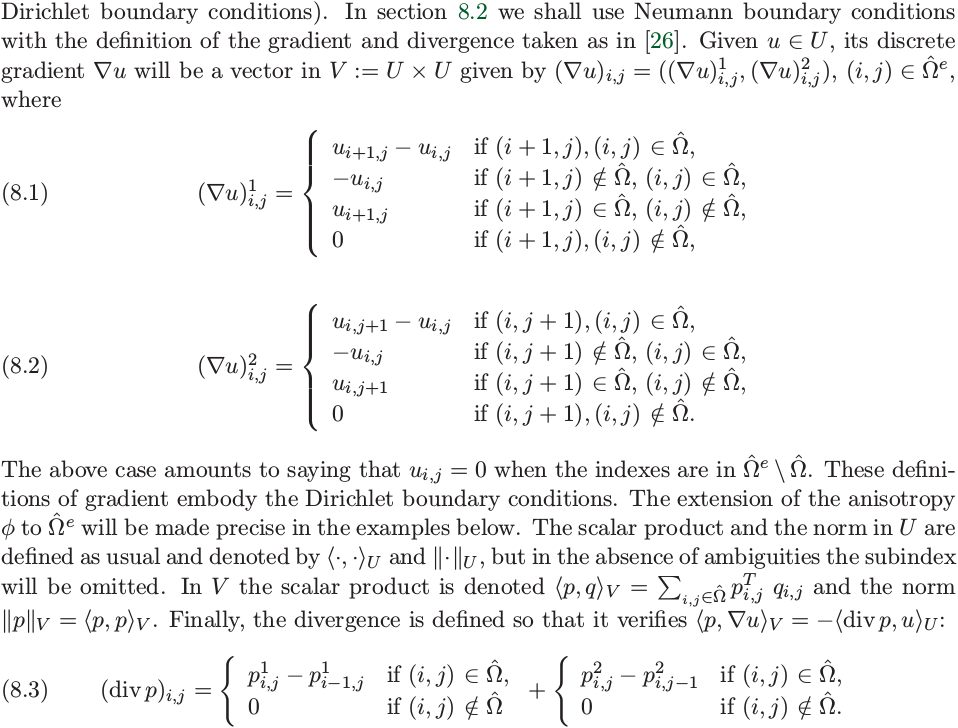
\includegraphics[width=0.85\linewidth]{f/horrific1.png}}
\end{frame}

\begin{frame}\tt
Horrific finite difference scheme {\rm \textnumero} 2\\
======================================\\
$ $\\
{\rm\tiny\color{gray}
J.~Weickert, K.~Hagenburg, M.~Breuß, and O.~Vogel\\
\emph{Linear Osmosis Models for Visual Computing}
2013 \\
}
	\fbox{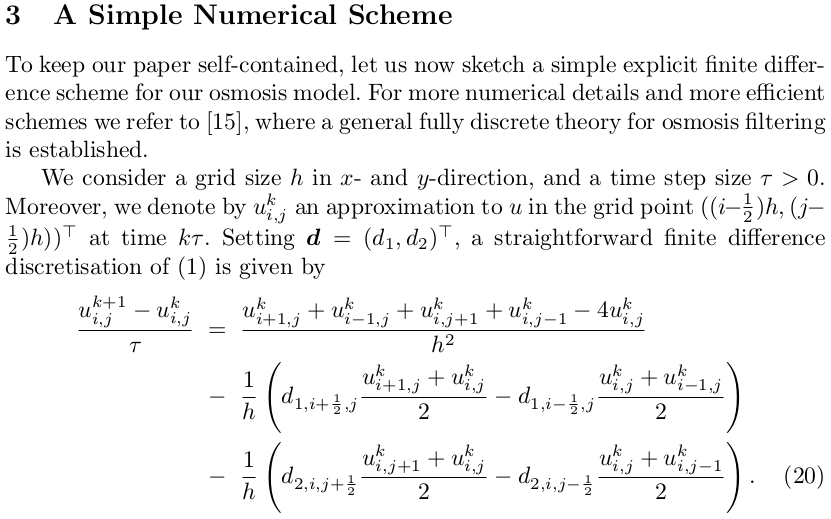
\includegraphics[width=0.65\linewidth]{f/divud.png}}
	\fbox{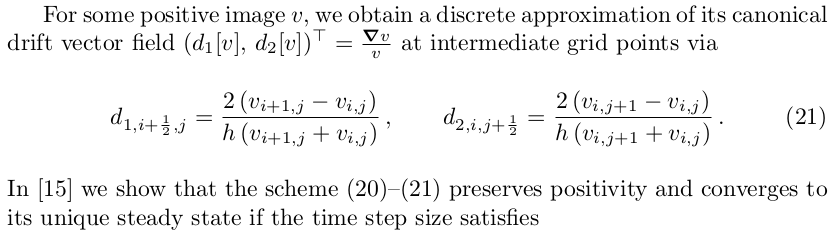
\includegraphics[width=0.65\linewidth]{f/divud2.png}}
\end{frame}

\begin{frame}\tt
Horrific finite difference scheme {\rm \textnumero} 3\\
======================================\\
$ $\\
{\rm\tiny\color{gray}
J.~Weickert, M.~Welk, M.~Wickert\\
\emph{$L^2$-Stable Nonstandard Finite Differences for Anisotropic Diffusion}
2013
	\\
}
\fbox{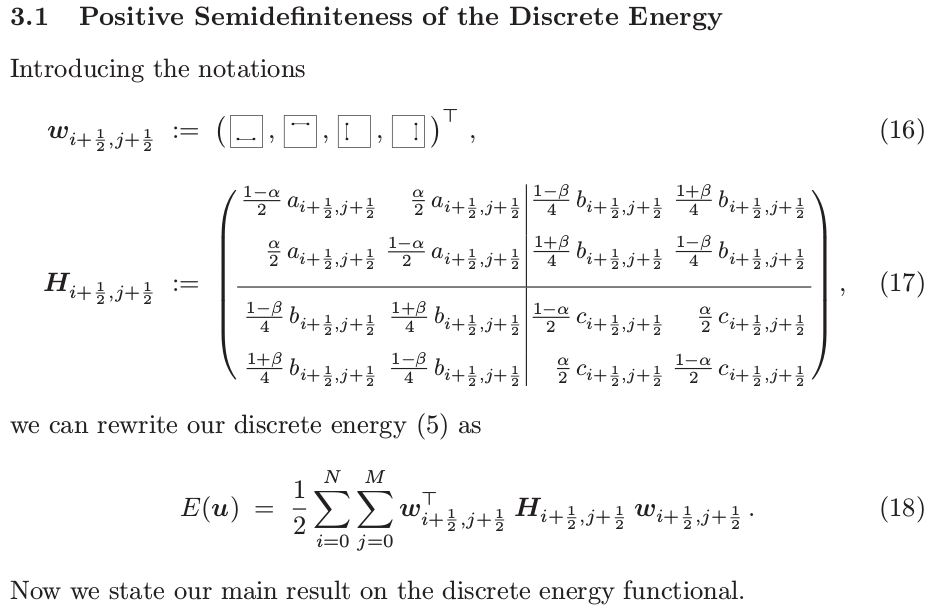
\includegraphics[width=0.85\linewidth]{f/weickerthell.png}}
\end{frame}


\begin{frame}\tt
(Not so much) horrific finite difference scheme {\rm \textnumero} 4\\
====================================================\\
$ $\\
{\rm\tiny\color{gray}
M.~di Martino, G.~Facciolo, E.~Meinhardt-Llopis\\
\emph{Poisson Image Editing}, IPOL 2016
	\\
}

\bigskip

\fbox{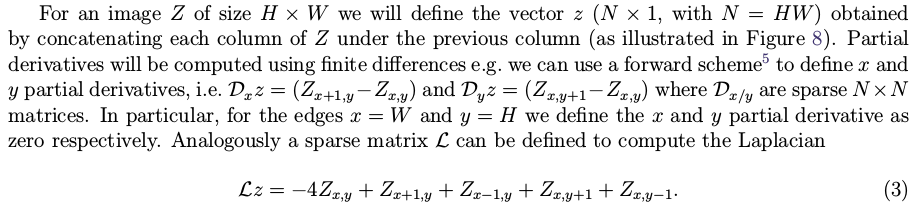
\includegraphics[width=0.95\linewidth]{f/poissonmatias.png}}
\end{frame}


%\begin{frame}[plain]\tt
%	\vfill
%	2. The correspondence between calculus and graph theory
%	\vfill
%\end{frame}
%
%
%\begin{frame}[fragile]
%%\includegraphics[width=3em]{f/archimedes.png}
%\begin{verbatim}MOTIVATION
%==========
%
%What would you tell Archimedes if you only had one minute?
%
%
%\end{verbatim}
%\pause
%\tt
%%The fundamental theorem of calculus, of course!
%
%The fundamental theorem of calculus\\
%-----------------------------------\\
%$ $\\
%A function $\mathbf{x}$ is a sequence of numbers: $x_1, x_2, x_3, \ldots$\\
%$\Delta\mathbf{x}_i := x_{i+1}-x_i\qquad\qquad\qquad$ (slope of the function)\\
%$\int_a^b\mathbf{x} := x_a+x_{a+1}+\cdots+x_{b-1}\qquad$ (area under the function)\\
%$ $\\
%{\bf Theorem:} $\int_a^b \Delta\mathbf{x}=x_b - x_a$\\
%
%\pause
%$ $\\
%\emph{Proof:}
%\only<3>{$(x_{a+1} - x_a) + (x_{a+2} - x_{a+1}) + \cdots + (x_{b-1}-x_{b-2}) + (x_b - x_{b-1})$}
%	\only<4>{$(\cancel{x_{a+1}} - x_a) + (\cancel{x_{a+2}} - \cancel{x_{a+1}}) + \cdots + (\cancel{x_{b-1}}-\cancel{x_{b-2}}) + (x_b - \cancel{x_{b-1}})$}
%\end{frame}


\begin{frame}[fragile]
%\includegraphics[width=3em]{f/archimedes.png}
\begin{verbatim}MOTIVATION: calculus of finite differences
==========================================

\end{verbatim}
	\begin{eqnarray*}
		\mathbf{x} &=& \ldots, x_1, x_2, x_3, \ldots \\
		\Delta\mathbf{x}_i  &=& x_{i+1} - x_i \\
		\Delta\mathbf{x}  &=& S\mathbf{x} - \mathbf{x} \\
		\Delta(a\mathbf{x}) &=& a\Delta\mathbf{x} \\
		\Delta(\mathbf{x}+\mathbf{y}) &=& \Delta\mathbf{x}+\Delta\mathbf{y} \\
		\sum_{a\le i <b}\Delta\mathbf{x}_i &=& x_b-x_a \\
		\Delta(\mathbf{xy}) &=&
			\mathbf{x}\Delta\mathbf{y}
			+\mathbf{y}\Delta\mathbf{x}
			+\Delta\mathbf{x}\Delta\mathbf{y}\\
			\pause
			&=&
			\mathbf{x}\Delta\mathbf{y}
			+S\mathbf{y}\Delta\mathbf{x}\\
			\pause
			&=&
			S\mathbf{x}\Delta\mathbf{y}
			+\mathbf{y}\Delta\mathbf{x}\\
			\pause
			&=&
			\mathbf{\widetilde{x}}\Delta\mathbf{y}
			+\mathbf{\widetilde{y}}\Delta\mathbf{x}
	\end{eqnarray*}

	\vfill
	where $\mathbf{\widetilde{x}} = \frac{S\mathbf{x}+\mathbf{x}}{2}$
\end{frame}

\begin{frame}[fragile]
\begin{verbatim}
RECALL OF VECTOR CALCULUS
=========================
\end{verbatim}
\tt
\setlength{\extrarowheight}{4pt}
\begin{tabular}{r|l}
	functions &
	$f:\R^2\to\R$
	\\
	vector fields &
	$\mathbf{v}:\R^2\to\R^2$
	\\
	gradient &
	$\nabla f=(f_x,f_y)$
	\\
	divergence&
	$\mathrm{div}(a,b)=a_x+b_y$
	\\
	laplacian&
	$\Delta f = \mathrm{div}(\nabla f) = f_{xx}+g_{yy}$
	\\
	product rule for gradient&
	$\nabla(fg)=f\nabla g+g\nabla f$
	\\
	product rule for divergence&
	$\mathrm{div}(f\mathbf{g})=f\mathrm{div}(\mathbf{g})+\mathbf{g}\cdot\nabla f$
	\\
	integral of $f$ on a domain&
	$\int_\Omega f$
	\\
	flux of $\mathbf{v}$ across a curve&
	$\int_S \mathbf{v}\cdot\mathbf{ds}$
	\\
	divergence theorem&
	$\int_{\partial\Omega}\mathbf{v}\cdot\mathbf{ds}=\int_\Omega\mathrm{div}(\mathbf{v})$
	\\
	energy functional &
	$E(u)=\int_\Omega L(u,Du,D^2u,\ldots)$
	\\
	Euler-Lagrange &
	$E'(u)=\frac{\partial L}{\partial u}
	-\mathrm{div}\frac{\partial L}{\partial D u}
	+\nabla^2\frac{\partial L}{\partial D^2 u}
	-\cdots$
	\\
\end{tabular}

\end{frame}

\begin{frame}[fragile]
\begin{verbatim}
RECALL OF GRAPH THEORY
======================

\end{verbatim}\tt

	A graph is $G=(V,E)$ where~$V\subseteq E\times E$.\\
	It is not directed: $(x,y)\in E\implies (y,x)\in E$.\\
	There are no loops~$(x,x)\not\in E$.

	\bigskip

	$n=\#V\ $ number of vertices,
	$\qquad V=\{1,\ldots,n\}$\\
	$m=\#E/2\ $ number of edges,
	$\qquad E=\{1,\ldots,m\}$\\

	\bigskip

	$A$ adjacency matrix ($n\times n$)\\
	$B$ signed incidence matrix ($m\times n$)\\
	$C=\frac{1}{2}|B|$ unsigned incidence matrix ($m\times n$)\\
	$L=-B^TB$ laplacian matrix ($n\times n$)

	\bigskip

	\pause
	\color{red}
	$\R^n$ functions defined on vertices\\
	$\R^m$ functions defined on edges\\

\end{frame}

\begin{frame}[fragile]
\begin{verbatim}
RECALL OF ALGEBRAIC GRAPH THEORY
================================

\end{verbatim}\tt

{\bf Observation:}
The graph matrices $A$, $B$, $C$, and $L$ can be interpreted as linear
	operators.
\bigskip

	Let~$f\in\R^n$ and~$\mathbf{g}\in\R^m$.  Then
	\medskip

	$Bf\in\R^m$ : $Bf(a,b) = f(b)-f(a)$\\

	\medskip

	$Cf\in\R^m$ : $\displaystyle Bf(a,b) = \frac{f(b)+f(a)}{2}$\\

	\medskip

	$Lf\in\R^n$ : $\displaystyle Lf(a) = \sum_{b\in N(a)}f(b)-f(a)$\\

	\medskip

	$-B^T\mathbf{g}\in\R^n$ : $-B^T\mathbf{g}(a)
	=\sum_{(a,b)\in E}\mathbf{v}(a,b)
	-\sum_{(b,a)\in E}\mathbf{v}(b,a)$

	\vfill
{\bf Observation 2:} From any of these matrices one can build all the others.

\end{frame}


\begin{frame}[fragile]
\begin{verbatim}THE CONTINUOUS / DISCRETE CORRESPONDENCE
========================================

\end{verbatim}
\scriptsize\tt
%\renewcommand{\arraystretch}{1.4}
\setlength{\extrarowheight}{3pt}
\begin{tabular}{l|l|b{0.3\textwidth}}
	\bf vector calculus & \bf graph theory & \bf octave code \\
	\hline
	euclidean plane $\R^2$ & graph $G=(V,E)$ &
	\begin{minted}[bgcolor=term,fontsize=\tiny]{octave}
		G = sparse(m,n);
	\end{minted}
	\\
	$p\in\R^2$ & $p\in V$ &
	\begin{minted}[bgcolor=term,fontsize=\tiny]{octave}
		i = randi(1, n);
	\end{minted}
	\\
	$v_p\in T_p\R^2$ & $v=(p,q)\in E$ &
	\begin{minted}[bgcolor=term,fontsize=\tiny]{octave}
		j = randi(1, m);
	\end{minted}
	\\
	$f:\R^2\to\R$ & $f:V\to\R$ &
	\begin{minted}[bgcolor=term,fontsize=\tiny]{octave}
		f = rand(1, n);
	\end{minted}
	\\
	$G:\R^2\to\R^2$ & $G:E\to\R$ &
	\begin{minted}[bgcolor=term,fontsize=\tiny]{octave}
		G = rand(1, m);
	\end{minted}
	\\
	$\mathfrak{X}^0\quad$ \color{gray}(functions) & $\R^n$ & \\
	$\mathfrak{X}^1\quad$ \color{gray}(fields) & $\R^m$ & \\
	$\nabla:\mathfrak{X}^0\to\mathfrak{X}^1$ & $B:\R^n\to\R^m$ &
	\begin{minted}[bgcolor=term,fontsize=\tiny]{octave}
		B = incidence(G);
	\end{minted}
	\\
	$\mathrm{div}:\mathfrak{X}^1\to\mathfrak{X}^0$ & $-B^T:\R^m\to\R^n$ &
	\begin{minted}[bgcolor=term,fontsize=\tiny]{octave}
		-B'
	\end{minted}
	\\
	$\Delta:\mathfrak{X}^0\to\mathfrak{X}^0$ & $-B^TB:\R^n\to\R^n$ &
	\begin{minted}[bgcolor=term,fontsize=\tiny]{octave}
		L = -B'*B;
	\end{minted}
	\\
	$\Omega\subseteq\R^2$, $\partial\Omega\subseteq\R^2$ & $\Omega\subseteq V$, $\partial\Omega\subseteq E$ &
	\begin{minted}[bgcolor=term,fontsize=\tiny]{octave}
		M = O>0; dM = -B*M;
	\end{minted}
	\\
	$\int_\Omega f$ & ${\mathbbm{1}_\Omega}^T f = \left\langle\mathbbm{1}_\Omega,f\right\rangle$ &
	\begin{minted}[bgcolor=term,fontsize=\tiny]{octave}
		M'*f
	\end{minted}
	\\
	$\int_{\partial\Omega}G=\int_\Omega\mathrm{div}G$ &
	$\left\langle -B\mathbbm{1}_{\Omega},G\right\rangle=\left\langle\mathbbm{1}_\Omega,-B^TG\right\rangle$ &
	\begin{minted}[bgcolor=term,fontsize=\tiny]{octave}
		(-B'*M)'*G == M'*(-B'*G)
	\end{minted}
	\\
	$fg$ & $f\odot g$ &
	\begin{minted}[bgcolor=term,fontsize=\tiny]{octave}
		f .* g == diag(f) * g
	\end{minted}
	\\
	$\nabla(fg)=f\nabla g+g\nabla f$ & $B(f\odot g)= ?$ &
	\begin{minted}[bgcolor=term,fontsize=\tiny]{octave}
		B * diag(f) * g == ?
	\end{minted}
	\\
\end{tabular}
\end{frame}

\begin{frame}[fragile]
\begin{verbatim}HADAMARD PRODUCT ASSOCIATIVITY
==============================

\end{verbatim}\tt
{\bf Lemma 1.}  Let $A$ be a $m\times n$ binary matrix with exactly one non-zero
	entry per row, and let $x,y\in\R^n$.  Then
\[
	A(x\odot y) = (Ax)\odot(Ay)% + y\odot A x
\]
{\it Proof.}
\(
	\displaystyle\sum_{\dot\jmath}a_{\dot\imath\dot\jmath}x_{\dot\jmath} y_{\dot\jmath}
	= a_{\dot\imath\hat\jmath}x_{\hat\jmath}y_{\hat\jmath}
	= a_{\dot\imath\hat\jmath}x_{\hat\jmath}\ a_{\dot\imath\hat\jmath}y_{\hat\jmath}
	= \sum_{\dot\jmath}a_{\dot\imath\dot\jmath}x_{\dot\jmath}
	\sum_{k}a_{\dot\imath k}y_k
	\)
\hfill\qedsymbol

\vfill
{\bf Lemma 2.}  Let~$B$ be the incidence matrix of a graph
	and~$C=\frac{1}{2}|B|$.  Then
\[
	B(x\odot y) = (Cx)\odot(By) + (Cy)\odot(Bx)
\]
{\it Proof.}  Decompose $B=B_1-B_2$ and apply Lemma 1.
\hfill\qedsymbol
\end{frame}

\begin{frame}[fragile]
\begin{verbatim}HADAMARD PRODUCT ASSOCIATIVITY
==============================

\end{verbatim}
{\bf Corollary (product rule for forward differences).}
	\[
		\Delta(\mathbf{xy}) = \mathbf{\widetilde{x}}\Delta\mathbf{y}
			+\mathbf{\widetilde{y}}\Delta\mathbf{x}
	\]
	where $\mathbf{\widetilde{x}} = \frac{S\mathbf{x}+\mathbf{x}}{2}$

	\bigskip

	{\bf Corollary (grad of product).}
	{\hfill\color{gray}$\nabla (fg) = f\nabla g+g\nabla f$}

	\medskip
	\begin{minted}[bgcolor=term]{octave}
		B * (f .* g)    ==    C*f .* B*g   +   C*g .* B.f
	\end{minted}

	\bigskip

	{\bf Corollary (div of product).}
	{\hfill\color{gray}$\mathrm{div}(fG)=f\mathrm{div}(G)+G\cdot\nabla f$}

	\medskip
	\begin{minted}[bgcolor=term]{octave}
		-B' * (C*f .* G)   ==  f .* (-B'*G)   +   C'*(B*f .* G)
	\end{minted}

\end{frame}

\begin{frame}[fragile]
\begin{verbatim}
DIFFERENTIAL GEOMETRY ON GRAPHS
===============================

\end{verbatim}
\setlength{\extrarowheight}{6pt}
\tt
\begin{tabular}{l|l}
	differential geometry & graph theory \\
	\hline
	manifold $M$ & graph $G=(V,E)$ \\
	$p\in M$ & $p\in v$ \\
	$v_p\in T_p'M$ & $v=(p,q)\in E$ \\
	$M$ & $V$ \\
	$T'M$ & $E$ \\
	$\Omega^0(M)$ & $\R^V$ \\
	$\Omega^1(M)$ & $\R^E$ \\
	$\Omega^p(M)$ & $\R^{\{p-1\ \textrm{cliques of G}\}}$ \\
	$d:\Omega^p(M)\to\Omega^{p+1}(M)$ & $B^{\wedge p}$ \\
	exterior algebra & Whitney clique complex \\
\end{tabular}
\end{frame}

%\begin{frame}[fragile]
%\begin{verbatim}
%ALGEBRAIC GRAPH THEORY IN MATLAB/OCTAVE
%=======================================
%
%\end{verbatim}
%\end{frame}
%
%\begin{frame}[fragile]
%\begin{verbatim}
%CORRESPONDENCE: points,vectors = vertices,edges
%===============================================
%
%\end{verbatim}\tt
%\begin{columns}[t,totalwidth=\linewidth]
%%	\begin{column}{0.5\linewidth}
%%		abc
%%
%%		lorem ipsum dolor si amet lorem ipsum dolor si amet lorem ipsum
%%		dolor si amet lorem ipsum dolor si amet lorem ipsum dolor si amet
%%		lorem ipsum dolor si amet lorem ipsum dolor si amet lorem ipsum
%%		dolor si amet lorem ipsum dolor si amet lorem ipsum dolor si amet
%%		lorem ipsum dolor si amet lorem ipsum dolor si amet lorem ipsum
%%		dolor si amet lorem ipsum dolor si amet lorem ipsum dolor si amet
%%	\end{column}
%%	\begin{column}{0.5\linewidth}
%%		lorem ipsum dolor si amet lorem ipsum dolor si amet lorem ipsum
%%		dolor si amet lorem ipsum dolor si amet lorem ipsum dolor si amet
%%		lorem ipsum dolor si amet lorem ipsum dolor si amet lorem ipsum
%%		dolor si amet lorem ipsum dolor si amet lorem ipsum dolor si amet
%%		lorem ipsum dolor si amet lorem ipsum dolor si amet lorem ipsum
%%		dolor si amet lorem ipsum dolor si amet lorem ipsum dolor si amet
%%	\end{column}
%	\begin{column}{0.5\linewidth}
%		plane $\R^2$
%
%		point $p\in\R^2$
%
%		vector $v_p\in T_p\R^2$
%
%		\bigskip
%
%		(figure of a tangent vector on a surface)
%	\end{column}
%	\vrule{}
%	\begin{column}{0.5\linewidth}
%		graph $G=(V,E)$
%
%		vertex $p\in V$
%
%		edge $v=(p,q)\in E$
%
%		%\usemodule[tikz]
%		\bigskip
%
%		(figure of a graph with stuff)
%		\usetikzlibrary{graphs}
%		\begin{tikzpicture}
%			\graph[nodes={draw,circle},edges={>=latex}] {
%				A [at={(0,0)}] -> {
%					B [at={(2,0)}] -> C [at={(2,-2)}],
%								  C -> D [at={(0,-2)},rectangle]
%									  }
%										};
%		\end{tikzpicture}
%	\end{column}
%\end{columns}
%\end{frame}
%
%\begin{frame}[fragile]
%\begin{verbatim}
%CORRESPONDENCE: points,vectors = vertices,edges
%===============================================
%
%\end{verbatim}\tt
%\begin{tabular}{p{0.5\linewidth}|p{0.5\linewidth}}
%	vector calculus & graph theory \\
%	\hline
%		plane $\R^2$
%
%		point $p\in\R^2$
%
%		vector $v_p\in T_p\R^2$
%
%		\bigskip
%
%		(figure of a tangent vector on a surface)
%		&
%		graph $G=(V,E)$
%
%		vertex $p\in V$
%
%		edge $v=(p,q)\in E$
%
%		%\usemodule[tikz]
%		\bigskip
%
%		(figure of a graph with stuff)
%		% tikz commented because it does not work
%		%\usetikzlibrary{graphs}
%		%\begin{tikzpicture}
%		%	\graph[nodes={draw,circle},edges={>=latex}] {
%		%		A [at={(0,0)}] -> {
%		%			B [at={(2,0)}] -> C [at={(2,-2)}],
%		%						  C -> D [at={(0,-2)},rectangle]
%		%							  }
%		%								};
%		%\end{tikzpicture}
%		\\
%\end{tabular}
%\end{frame}
%
%\begin{frame}[fragile]
%\begin{verbatim}
%CORRESPONDENCE: scalar and vector fields
%========================================
%
%\end{verbatim}\tt
%\begin{columns}[t,totalwidth=\linewidth]
%	\begin{column}{0.5\linewidth}
%		scalar field $f:\R^2\to\R$
%
%		{\color{gray}(co)-}vector field $F:\R^2\to\R^2$
%
%		\bigskip
%
%		(figure of a scalar and a vector field on the plane)
%	\end{column}
%	\begin{column}{0.5\linewidth}
%		scalar field $f:V\to\R$
%
%		vector field $F:E\to\R$
%
%		$f\in\R^n\qquad F\in\R^m$
%		\bigskip
%
%		(figure of a graph with numbers on edges and vertices)
%	\end{column}
%\end{columns}
%	\color{gray}note on fields and forms
%\end{frame}
%
%\begin{frame}[fragile]
%\begin{verbatim}
%CORRESPONDENCE: the gradient
%============================
%
%\end{verbatim}
%\end{frame}
%
%\begin{frame}[fragile]
%\begin{verbatim}
%CORRESPONDENCE: the divergence
%==============================
%
%\end{verbatim}
%\end{frame}
%
%\begin{frame}[fragile]
%\begin{verbatim}
%CORRESPONDENCE: the laplacian
%=============================
%
%\end{verbatim}
%\end{frame}
%
%\begin{frame}[fragile]
%\begin{verbatim}
%CORRESPONDENCE: the centering operator
%======================================
%
%\end{verbatim}
%\end{frame}
%
%\begin{frame}[fragile]
%\begin{verbatim}
%CORRESPONDENCE: the diffusion operator
%======================================
%
%\end{verbatim}
%\end{frame}
%
%\begin{frame}[fragile]
%\begin{verbatim}
%CORRESPONDENCE: pointwise product / hadamard product
%====================================================
%
%\end{verbatim}
%\end{frame}
%
%\begin{frame}[fragile]
%\begin{verbatim}
%CORRESPONDENCE: Leibniz rules
%=============================
%
%\end{verbatim}
%\end{frame}
%
%\begin{frame}[fragile]
%\begin{verbatim}
%CORRESPONDENCE: integrals
%=========================
%
%\end{verbatim}
%\end{frame}
%
%\begin{frame}[fragile]
%\begin{verbatim}
%CORRESPONDENCE: boundaries
%==========================
%
%\end{verbatim}
%\end{frame}
%
%\begin{frame}[fragile]
%\begin{verbatim}
%CORRESPONDENCE: Stokes theorem
%==============================
%
%\end{verbatim}
%\end{frame}
%
%\begin{frame}[fragile]
%\begin{verbatim}
%CORRESPONDENCE: partial differential equatio
%==============================================
%
%\end{verbatim}
%\end{frame}
%
%\begin{frame}[fragile]
%\begin{verbatim}
%CORRESPONDENCE: Neumann boundary conditions
%===========================================
%
%\end{verbatim}
%\end{frame}
%
%\begin{frame}[fragile]
%\begin{verbatim}
%CORRESPONDENCE: Dirichlet boundary conditions
%=============================================
%
%\end{verbatim}
%\end{frame}
%
%\begin{frame}[fragile]
%\begin{verbatim}
%CORRESPONDENCE: the osmosis equation
%====================================
%
%\end{verbatim}
%\end{frame}
%
%\begin{frame}[fragile]
%\begin{verbatim}
%RECALL: minimzation of quadratic forms
%======================================
%
%\end{verbatim}\tt
%	Let $A\in\mathcal{M}_n(\R)$ be a symmetric positive definite matrix and let~$b\in\R^n$.  Then the function
%	\begin{eqnarray*}
%		f :& \R &\to \R\\
%		   & x &\mapsto f(x)=\frac{1}{2}x^TAx-b^Tx
%	\end{eqnarray*}
%	has a unique minimum $x\in\R^n$.  Moreover, this minimum is the unique
%	solution of the equation
%	\[
%		Ax=b
%	\]
%\end{frame}
%
%\begin{frame}[fragile]
%\begin{verbatim}
%CORRESPONDENCE: variational interpretation
%==========================================
%
%\end{verbatim}
%\end{frame}
%
%\begin{frame}[fragile]
%\begin{verbatim}
%CORRESPONDENCE: non-uniformities and anisotropies
%=================================================
%
%\end{verbatim}
%\end{frame}
%
%\begin{frame}[fragile]
%\begin{verbatim}
%SUCCESSFUL EXAMPLE: variational osmosis
%=======================================
%
%\end{verbatim}
%\end{frame}

\begin{frame}[fragile]
\begin{verbatim}
EXAMPLE: smoothing the streets of London
========================================

\end{verbatim}

\tt Woolwich tunnel

\only<1>{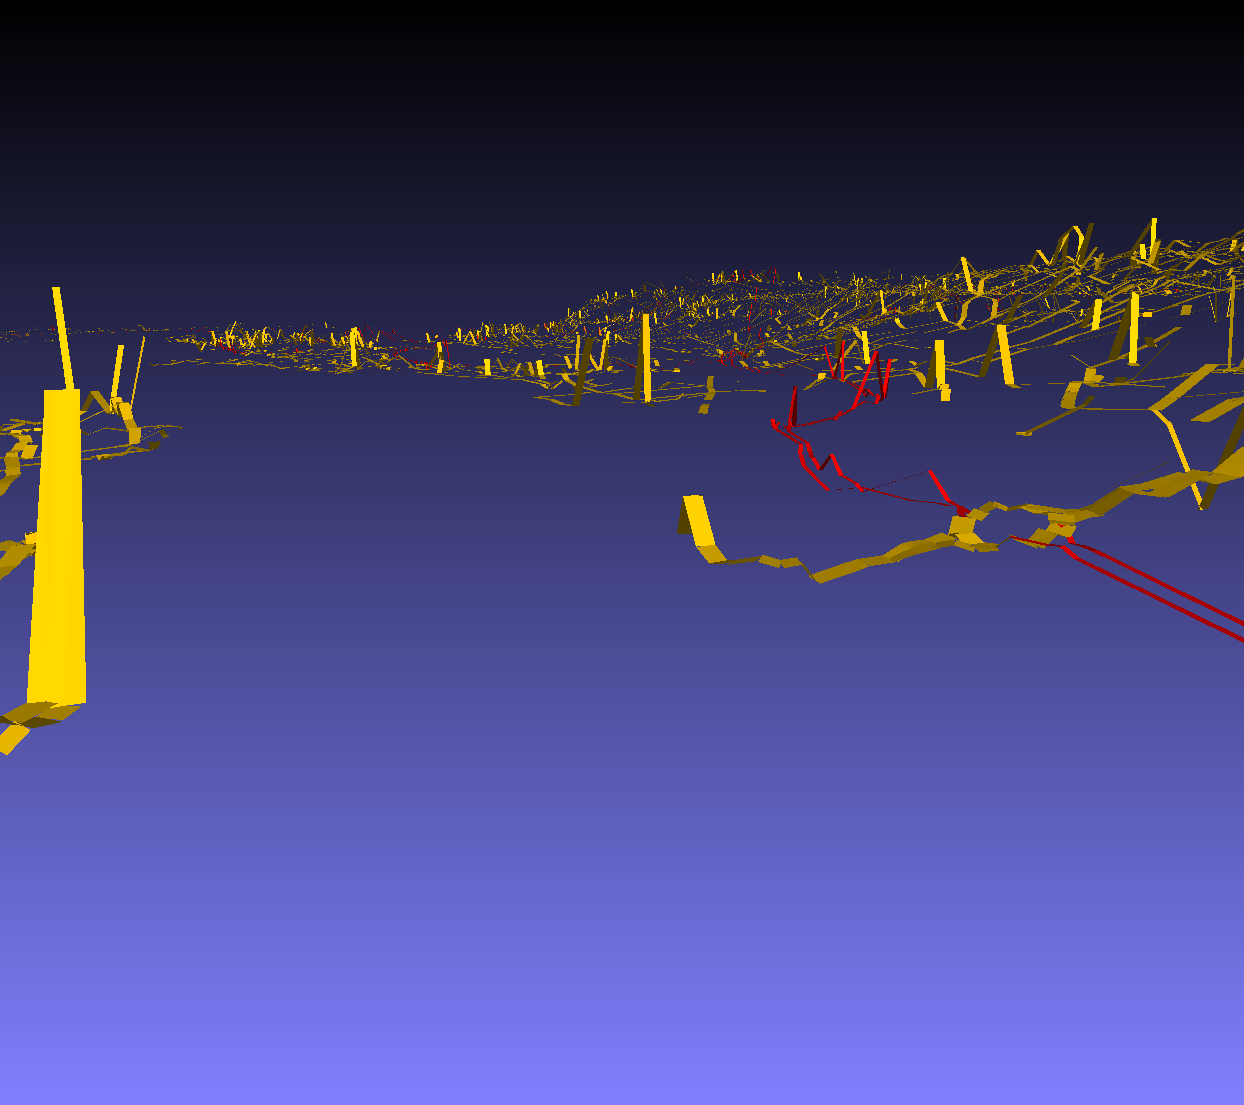
\includegraphics[height=0.7\textheight]{fb/woolwich_before.png}}%
\only<2>{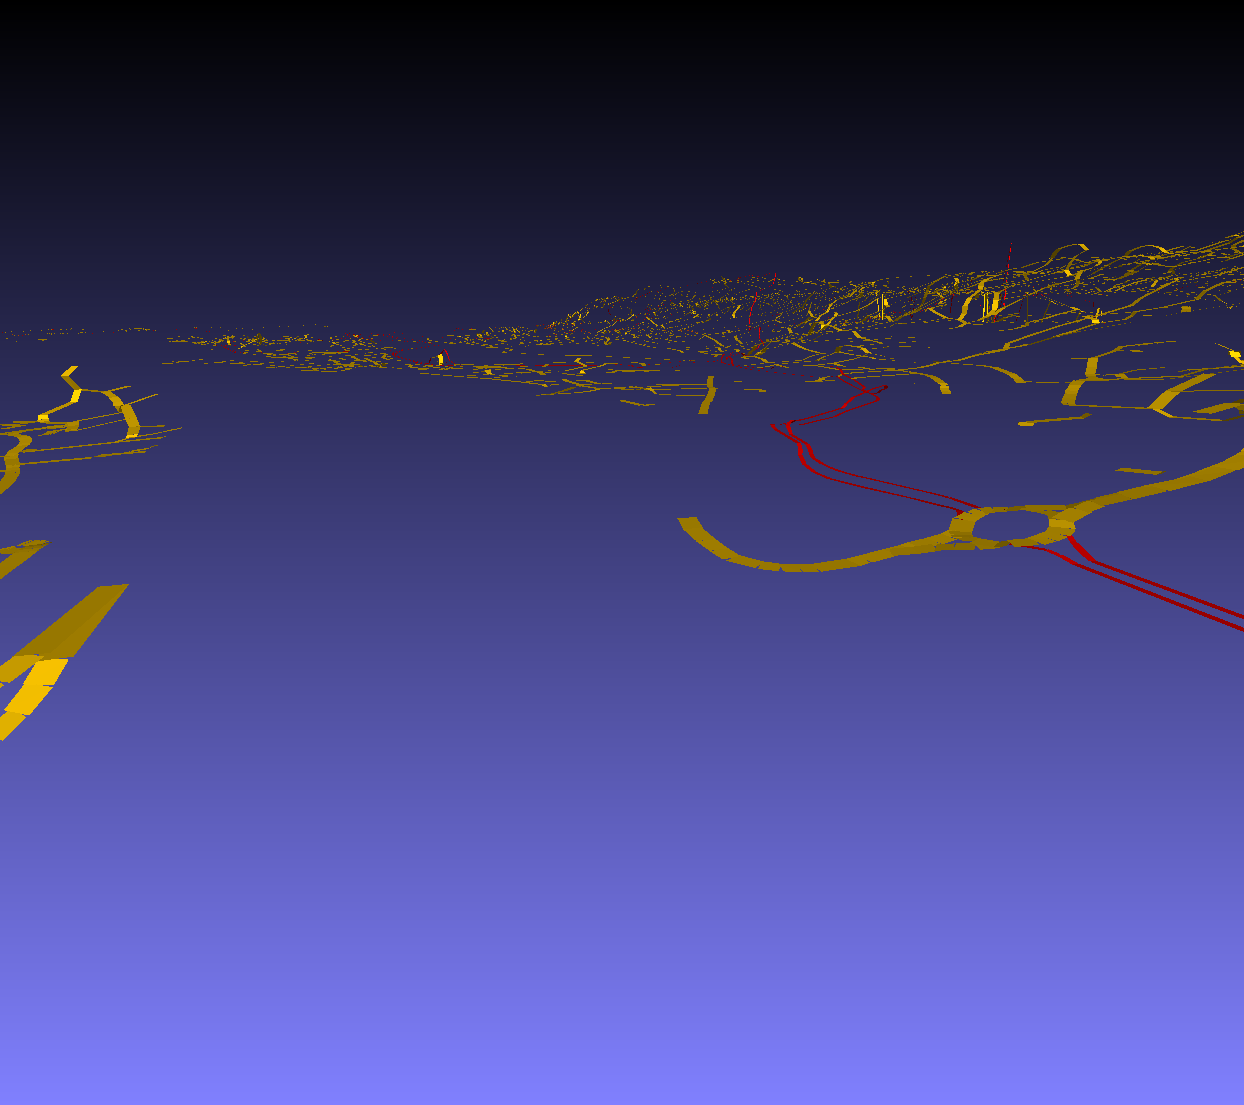
\includegraphics[height=0.7\textheight]{fb/woolwich_after.png}}%
\end{frame}

\begin{frame}[fragile]
\begin{verbatim}
EXAMPLE: smoothing the streets of London
========================================

\end{verbatim}

\tt Woolwich tunnel closeup

\only<1>{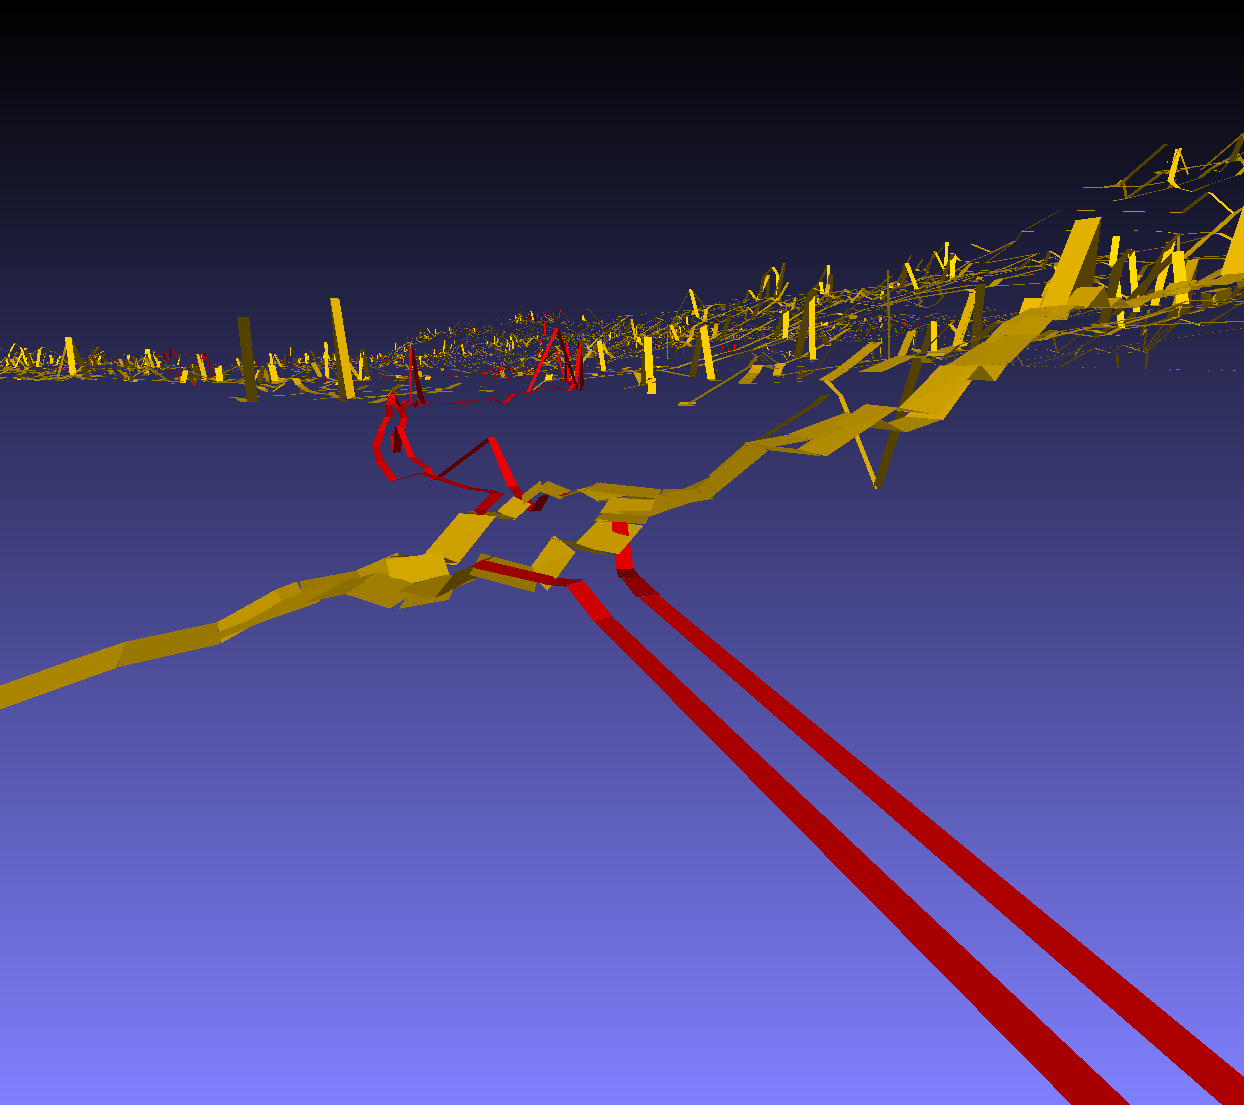
\includegraphics[height=0.7\textheight]{fb/wool1_before.png}}%
\only<2>{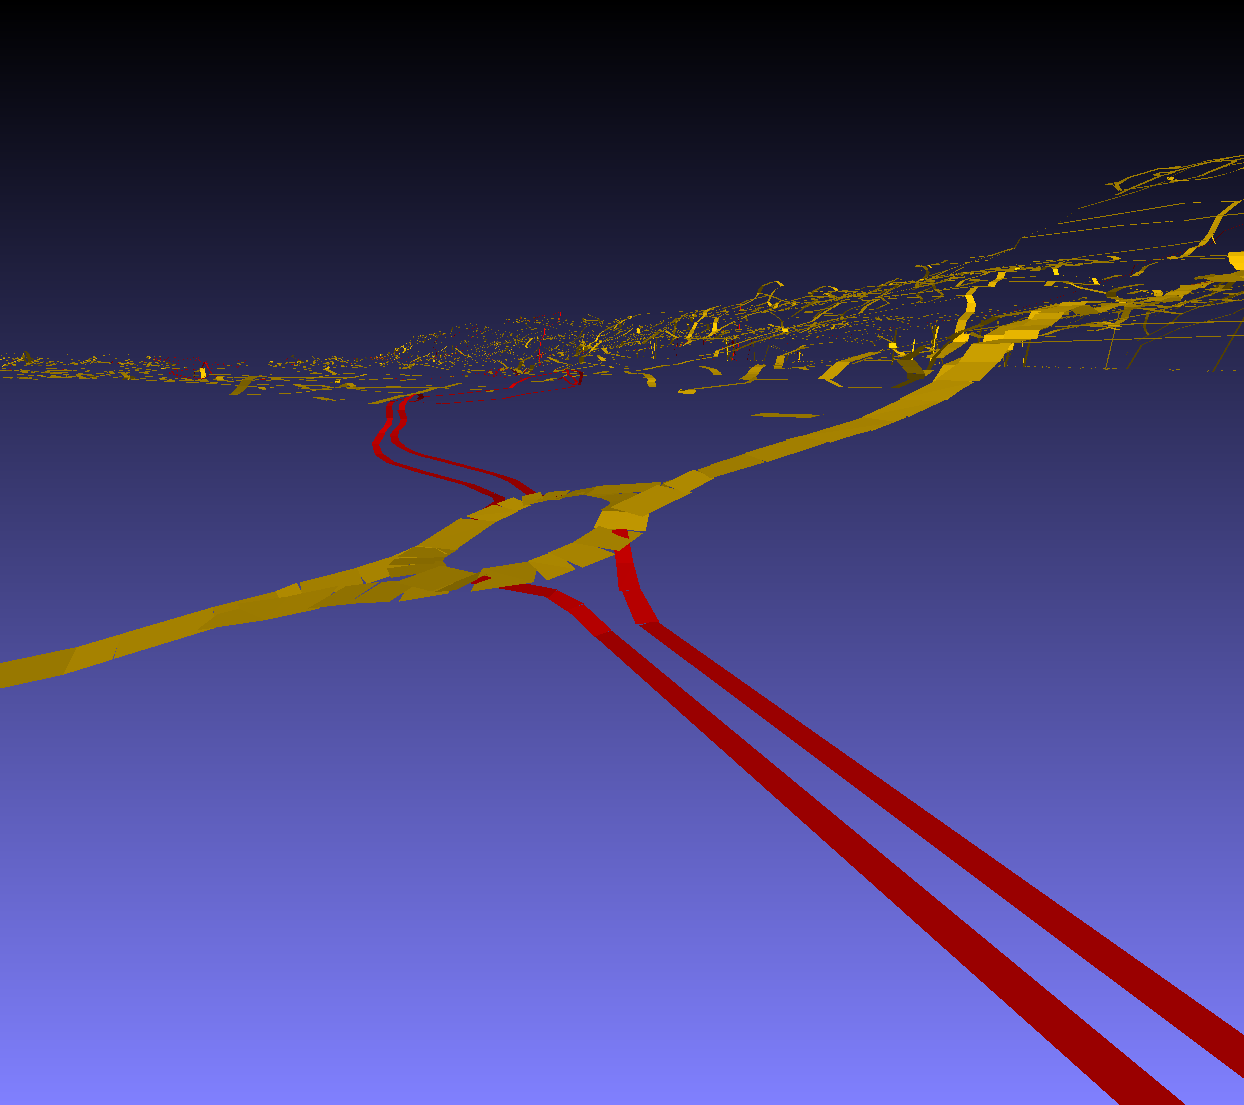
\includegraphics[height=0.7\textheight]{fb/wool1_after.png}}%
\end{frame}


\begin{frame}[fragile]
\begin{verbatim}
EXAMPLE: smoothing the streets of London
========================================

\end{verbatim}

\tt Shooter's hill

\only<1>{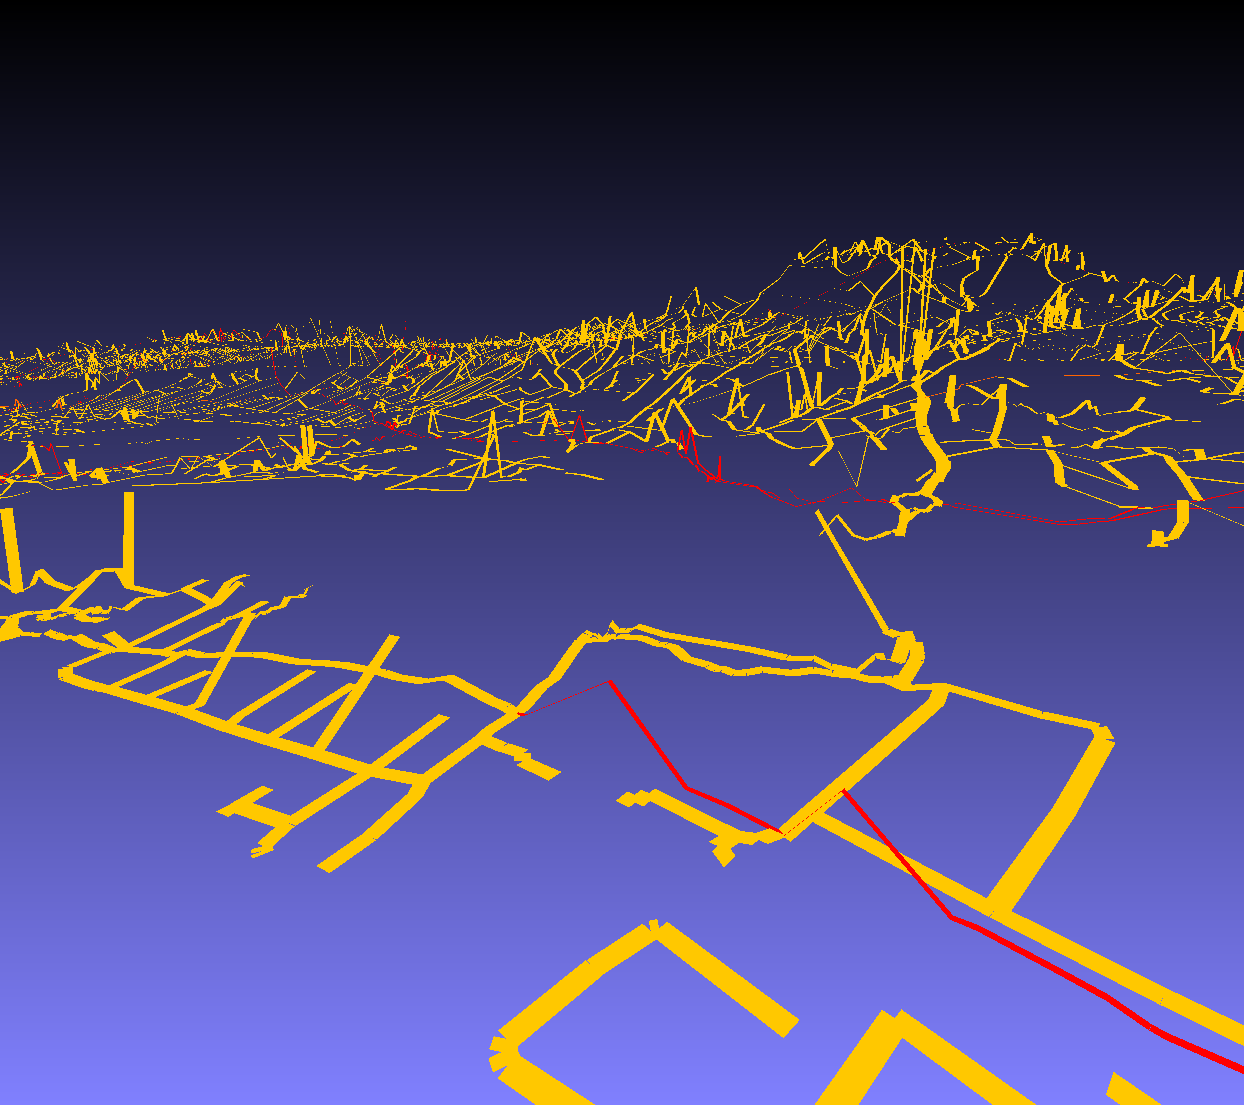
\includegraphics[height=0.7\textheight]{fb/hill_before.png}}%
\only<2>{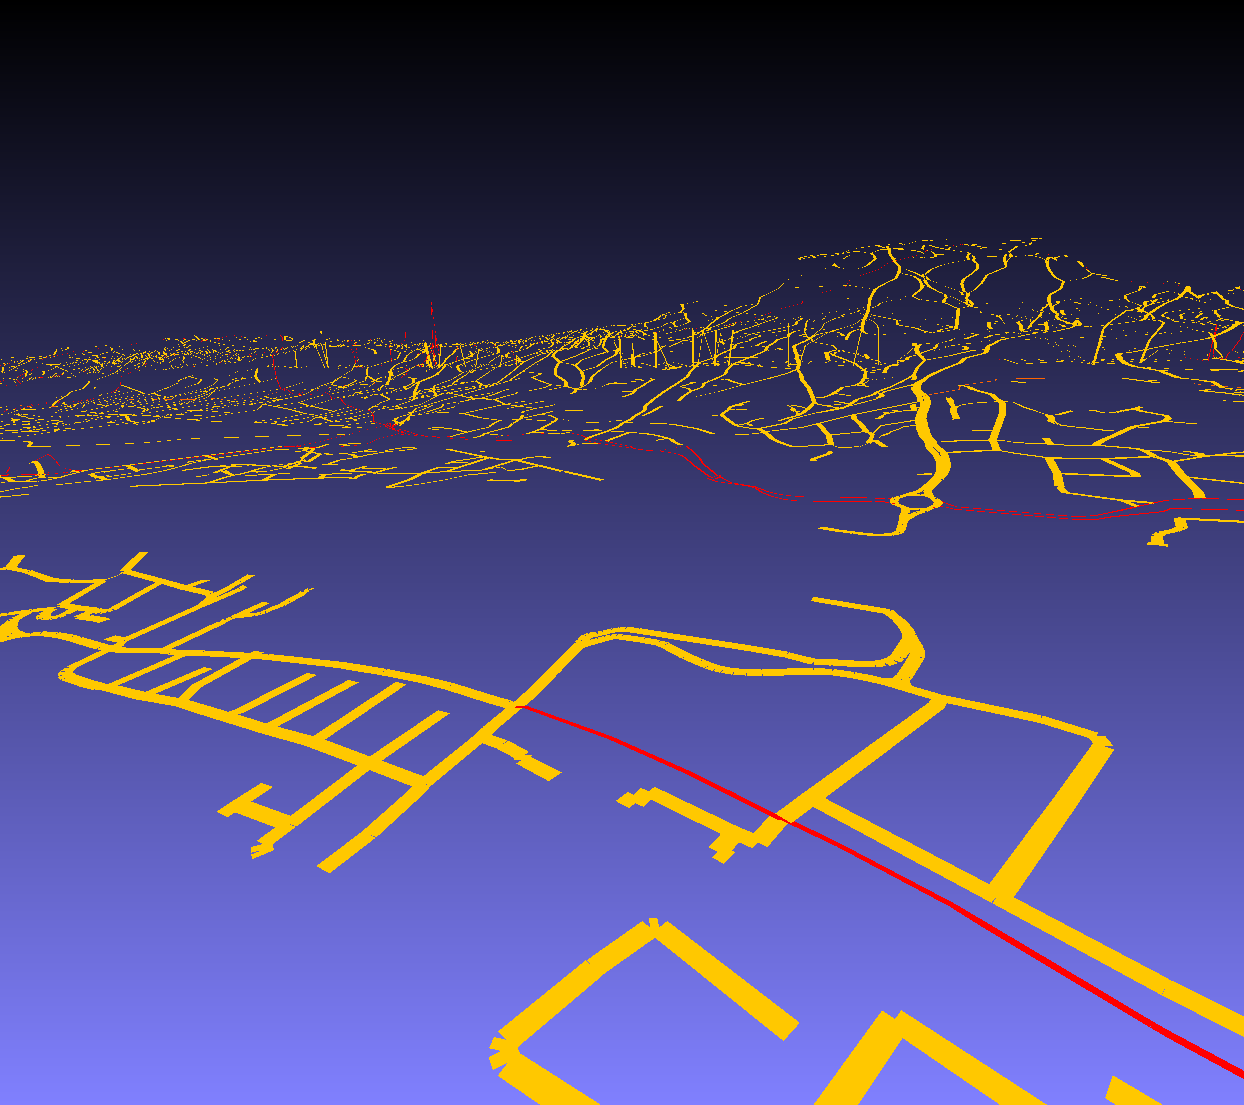
\includegraphics[height=0.7\textheight]{fb/hill_after.png}}%
\end{frame}

\begin{frame}[fragile]
\begin{verbatim}
EXAMPLE: smoothing the streets of London
========================================

\end{verbatim}
\begin{minted}[frame=single,fontsize=\tiny]{octave}
# Process the London roadmap

# 1. load the raw data of the graph
nodes   = dlmread("nodes.txt");
edges   = dlmread("roads.txt");
heights = dlmread("heights.txt");

# 2. extract raw data into user-friendly variables
n = size(nodes, 1);      # number of vertices
m = size(edges, 1);      # number of edges
e_from = 1 + edges(:,2);
e_to   = 1 + edges(:,3);

# 3. build incidence matrix B
Bfrom = sparse(1:m, e_from, 1, m, n);
Bto   = sparse(1:m, e_to  , 1, m, n);
B = Bto - Bfrom;

# 4. build laplacian matrix L
L = -B'*B;

# 5. solve the heat equation
t  = 1;
h  = expm(t * L) * heights;

# 6. save the result
dlmwrite("heights_smooth.txt", h);
\end{minted}
\end{frame}

\begin{frame}[fragile]
\begin{verbatim}
EXAMPLE: smoothing the streets of London
========================================

\end{verbatim}

\begin{minted}[frame=single,fontsize=\small]{octave}
# 5'. approximate the heat equation
tau = 0.24;
h = heights
for i = 1:9
        h += tau * (L * h);
end
\end{minted}

\vfill

\begin{minted}[frame=single,fontsize=\small]{octave}
# 3'. weighted incidence matrix
weights  = raw_edges(:,4);
B = sqrt(weights) .* (Bto - Bfrom);
\end{minted}

\vfill
\end{frame}

\begin{frame}[fragile]
\begin{verbatim}
EXAMPLE: Poisson equation with Dirichlet B.C.
=============================================

\end{verbatim}
\tiny\tt
\begin{tabular}{cc}
	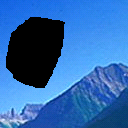
\includegraphics[height=0.3\textheight]{lenasky/crop_lenasky_boundary.png} &
	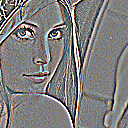
\includegraphics[height=0.3\textheight]{lenasky/crop_minuslap.png} \\
	boundary condition &
	laplacian \\
	& \\
	& \\
	& \\
	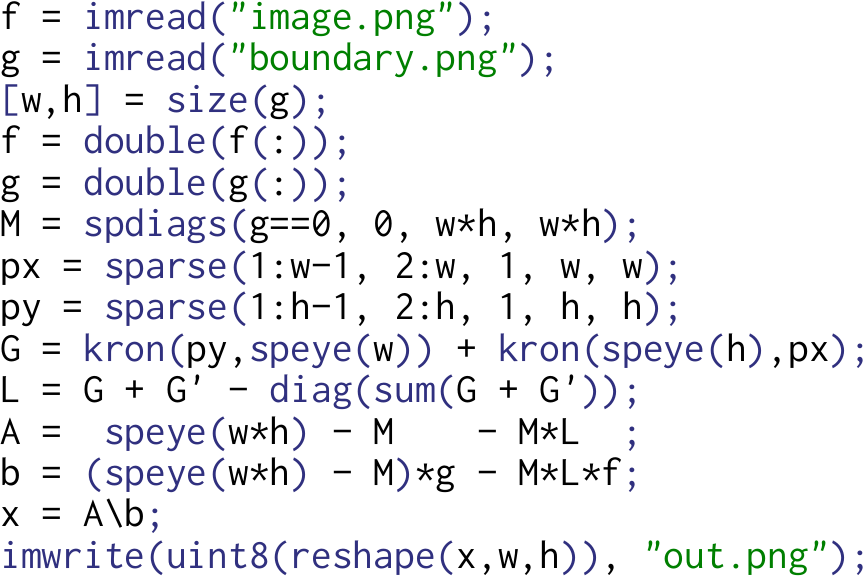
\includegraphics[height=0.3\textheight]{lenasky/miniercode.png} &
	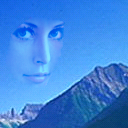
\includegraphics[height=0.3\textheight]{lenasky/crop_result.png} \\
	poisson solver &
	result \\
\end{tabular}
\end{frame}

\begin{frame}[fragile]
\begin{verbatim}
EXAMPLE: Poisson equation with Dirichlet B.C.
=============================================

\end{verbatim}\tt
\begin{minted}[frame=single,fontsize=\tiny]{octave}
# read input
f = imread("lena.png");
g = imread("landscape.png");
[w,h] = size(g);
f = double(f(:));
g = double(g(:));

# build mask operator
M = spdiags(g==0, 0, w*h, w*h);

# build laplacian operator on the whole image
px = sparse(1:w-1, 2:w, 1, w, w);
py = sparse(1:h-1, 2:h, 1, h, h);
G = kron(py,speye(w)) + kron(speye(h),px);
L = G + G' - diag(sum(G + G'));

# compute laplacian of the image to paste
Lf = L*f;

# state the problem
I = speye(w*h)
A =  I - M    - M*L ;
b = (I - M)*g - M*Lf;

# solve the problem
x = A\b;

# write output
imwrite(uint8(reshape(x,w,h)), "out.png");
\end{minted}
\end{frame}

\begin{frame}[fragile]
\begin{verbatim}
EXAMPLE: Weickert's "non-standard" scheme
=========================================

\end{verbatim}\tt

\vfill

\fbox{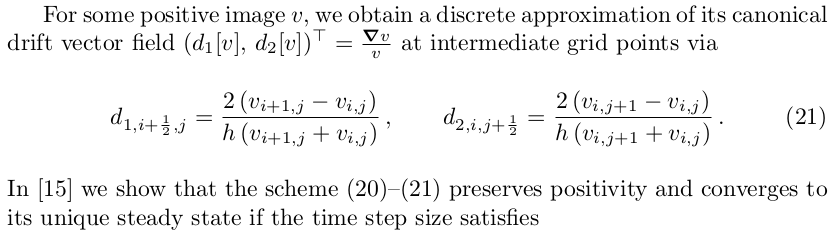
\includegraphics[width=0.85\linewidth]{f/divud2.png}}

\vfill

This is simply $$d=\frac{1}{Cv}\odot Bv$$

\vfill

\end{frame}

\begin{frame}[fragile]
\begin{verbatim}
UNEXPECTED DIFFICULTIES: non-unique discretizations
===================================================

\end{verbatim}
	\tt How to discretize~$d=\frac{\nabla u}{u}$ ?

	\bigskip

\begin{enumerate}
	\item Standard: $d=\frac{1}{Cu}\odot Bu$
	\item Alternative: $d= C\frac{1}{u}\odot Bu$
	\item Logarithmic: $d=B \log(u)$
	\item Strange: $d=C(\frac{1}{u}\odot C^TB u)$
\end{enumerate}
\end{frame}

%\begin{frame}[fragile]
%\begin{verbatim}
%ALTERNATIVE: NON-GRAPHICAL DISCRETIZATION
%=========================================
%
%Pixels are not a graph.
%
%They are very small squares on the plane.
%
%This plane is endowed with a piecewise constant metric.
%\end{verbatim}
%\end{frame}

% missing frames
%
% * note: recall of vector calculus
% * note: recall of graph theory
% * note: recall of algebraic graph theory
% * note: algebraic graph theory in matlab/octave
% * correspondence: points,vectors = verrices,edges
% * correspondence: scalar fields, vector fields
% * correspondence: the gradient (B)
% * correspondence: the divergence (-B')
% * correspondence: the laplacian (L=-B'*B)
% * correspondence: centering operator (C=abs(B)/2)
% * correspondence: diffusion operator (C'*C)
% * correspondence: pointwise product / hadamard product (.*)
% * correspondence: leibniz rules
% * correspondence: integrals
% * correspondence: boundaries
% * correspondence: stokes theorem
% * correspondence: EDPs, general case, poisson example
% * correspondence: EDPs, neumann conditions
% * correspondence: EDPs, dirichlet conditions
% * correspondence: EDPs, osmosis
% * note: minimization of a quadratic form
% * correspondence: the variational interpretation: poisson, various cases
% * correspondence: anisotropies

\begin{frame}[fragile]
\begin{verbatim}
BIBLIOGRAPHY
============

* Folklore (people who know, think that everybody else does)

* Gabriel Peyré: numerical tours
* Olivier Lezoray: image processing and analysis with graphs
* Yves Colin de Verdière: spectres de graphes, ...
* Leo Grady and Jonathan Polimeni: discrete calculus

* Anil Hirani: discrete exterior calculus

* Oliver Knill: quantum calculus

* Penrose, Rovelli, Baez: discrete mechanics, spin foams, ...

\end{verbatim}
\end{frame}

\end{document}


% vim:sw=4 ts=4 spell spelllang=en:
